\documentclass{ou-report}
\citestyle{agu}

% Dit template is gemaakt door P.J. Molijn in het kader van zijn afstuderen aan de OU in 2014.
% Waarvoor hartelijk dank.
% Minieme maar belangrijke wijzigingen zijn aangebracht door E.M. van Doorn
% Het template is versimpeld door Sylvia Stuurman, 2019.


%\hypersetup{
%pdfsubject={Master Thesis <Titel>, <author>},
%pdfkeywords={keyword1, keyword2}
%}

\begin{document}
\pagestyle{plain}
\title{Dit is de titel van mijn}
\author{Ik ben de auteur}
%Title of the thesis
%\title[Subtitle]{Title}
%\author{author}
%\affiliation{
%\begin{tabular}{ll}
%Student: & studentnumber \\
%Date:    & DD/MM/YYY \\
%\end{tabular}
%}
%
%%\coverimage{cover/cover.jpg}
%%            ===============
%\makecover[frontboxwidth=4.6in]
\begin{titlepage}

    \begin{center}

        %% Insert the OU logo at the bottom of the page.
        \begin{tikzpicture}[remember picture,overlay]
            \node at (current page.south)[anchor=south,inner sep=0pt]{
                
\includegraphics[scale=0.7]{cover/logo}
            };
        \end{tikzpicture}

        %% Extra whitespace at the top.
        \vspace*{2\bigskipamount}

        %% Print the title in specific color.
        {\makeatletter
            %\titlestyle\color{ou-cyan}\Huge\@title
            \titlestyle\color{red}\Huge\@title
            \makeatother}

        %% Print the optional subtitle in black.
        {\makeatletter
            \ifx\@subtitle\undefined\else
                \bigskip
                \titlefont\titleshape\LARGE\@subtitle
            \fi
            \makeatother}

        \bigskip
        \bigskip

        by
        %door

        \bigskip
        \bigskip

        %% Print the name of the author.
        {\makeatletter
            \titlefont\Large\bfseries\@author
            \makeatother}

        \vfill

        in partial fulfillment of the requirements for the degree of
        %in overeenstemming met de vereisten voor het verkrijgen van de graad van

        \bigskip
        \bigskip

        {\bfseries Master of Science}

        in Software Engineering

        \bigskip
        \bigskip

        at the Open University, faculty of Management, Science and Technology \\
        Master Software Engineering
        %aan de Open Universiteit Nederland,

        to be defended publicly on 12 October, 2023 at 9:30 AM.
        %in het openbaar te verdedigen op dinsdag 9 september om 15:00 uur.

        \vfill

        \begin{tabular}{lll}
            %% Add additional information here, per faculty requirements, e.g
            Student number: & 852372917                                                 \\
            Course code:    & IMA0002                                                   \\
            Thesis committee:
                            & Dr. Ir. Mina Sheikhalishahi (chairman), & Open University \\
                            & Dr. Ir. Clara Maathuis (supervisor),    & Open University
        \end{tabular}

        %% Only include the following lines if confidentiality is applicable.
        \bigskip


        \bigskip

    \end{center}

\end{titlepage}


%% Use Roman numerals for the page numbers of the title pages and table of
%% contents.
\pagenumbering{roman}
%% Include an optional title page.

\frontmatter


\let\cleardoublepage\clearpage

% Optional Dedication, Acknowledgement
%\input{dedication}

%\input{acknowledgement}
\tableofcontents

%Optional: list of figures, list of tables
%\listoffigures

%\listoftables

%% Include an optional summary page.
%\chapter{Summary}

%\input{Summary/samenvatting}

\mainmatter
\pagenumbering{arabic}

\chapter{Title of the chapter}
This is just to show how to include a test file for a chapter, a reference \cite{ledesma_scree_2015}

%\input{Chapter2/chapter-2}

%\input{Chapter3/chapter-3}

%\input{Chapter4/chapter-4}

%\input{Chapter5/chapter-5}

%\input{Chapter6/chapter-6}



\backmatter
\pagenumbering{roman}

\bibliographystyle{plainnat}
\bibliography{report}

%% Use letters for the chapter numbers of the appendices.
%\appendix
\appendix
%  \chapter{Hyperparameters}
\section{K-Means}
For selecting the appropriate amount of clusters, we used the silhouette method. 
Using this method, we ran the K-Means method multiple times for different $k$ values.
The results are plotted using a line-plot, and we select the highest silhouette score from this plot. 
\begin{enumerate}
  \item Seeds dataset (All dimensions): k-clusters.
  \begin{enumerate}
      \item 2-dimensions k-value: 2
      \item 3-dimensions k-value: 5
      \item 7-dimensions k-value: 2
  \end{enumerate}
      \item Heart dataset:
      \begin{enumerate}
          \item 2-dimensions k-value: 2
          \item 3-dimensions k-value: 4
          \item 9-dimensions k-value: 2
      \end{enumerate}
      \item Circle dataset:
      \begin{enumerate}
          \item 2-dimensions k-value: 7
          \item 3-dimensions k-value: 9
      \end{enumerate}
      \item Line dataset:
      \begin{enumerate}
          \item 2-dimensions k-value: 2
          \item 3-dimensions k-value: 2
      \end{enumerate}
      \item Skewed dataset:
      \begin{enumerate}
          \item 2-dimensions k-value: 5
          \item 3-dimensions k-value: 4
      \end{enumerate}
  \end{enumerate}

\newpage
\subsection{Seeds dataset}
\begin{figure}[H]
  \includegraphics[width=0.75\textwidth]{Method/images//k-values/seeds-dataset-2-kmeans.png}
  \caption{Selecting the $k$ for K-Means clustering for seeds dataset (2 dimensions) using the "silhouette method"}
  \label{hyperparameters:agglomerative-seeds-dataset-2d}
\end{figure}
\begin{figure}[H]
  \includegraphics[width=0.75\textwidth]{Method/images/k-values/seeds-dataset-2-kmeans.png}
  \caption{Selecting the $k$ for K-Means clustering for seeds dataset (3 dimensions) using the "silhouette method"}
  \label{hyperparameters:agglomerative-seeds-dataset-3d}
\end{figure}
\begin{figure}[H]
  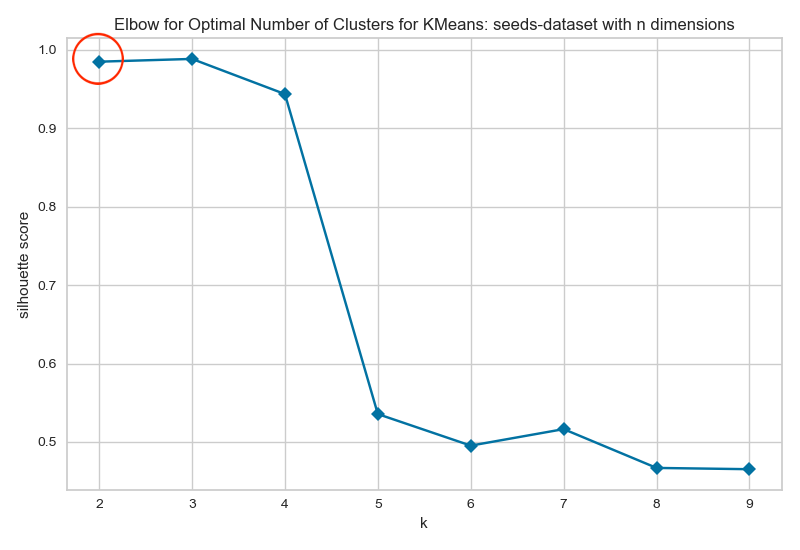
\includegraphics[width=0.75\textwidth]{Method/images/k-values/seeds-dataset-n-kmeans.png}
  \caption{Selecting the $k$ for K-Means clustering for seeds dataset (7 dimensions) using the "silhouette method"}
  \label{hyperparameters:agglomerative-seeds-dataset-7d}
\end{figure}
\newpage

\subsection{Heart dataset}
\begin{figure}[H]
  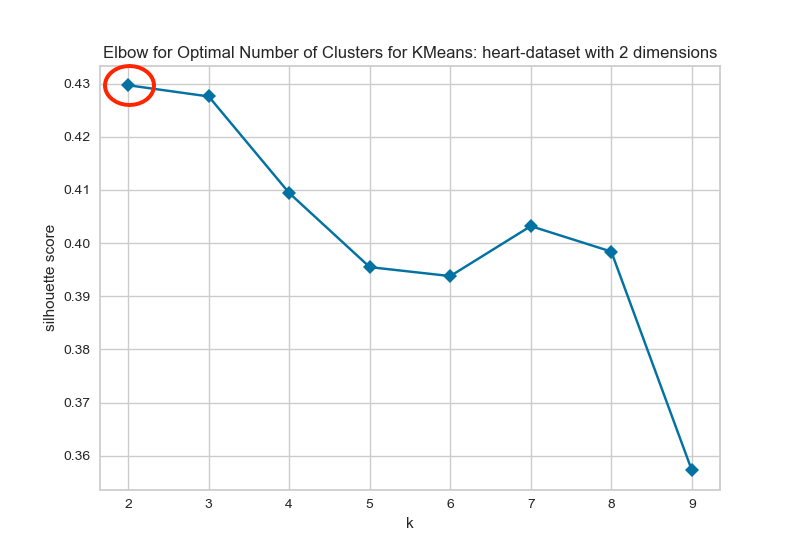
\includegraphics[width=0.75\textwidth]{Method/images/k-values/heart-dataset-2-kmeans.png}
  \caption{Selecting the $k$ for K-Means clustering for Heart dataset (2 dimensions) using the "silhouette method"}
  \label{hyperparameters:agglomerative-heart-dataset-2d}
\end{figure}
\begin{figure}[H]
  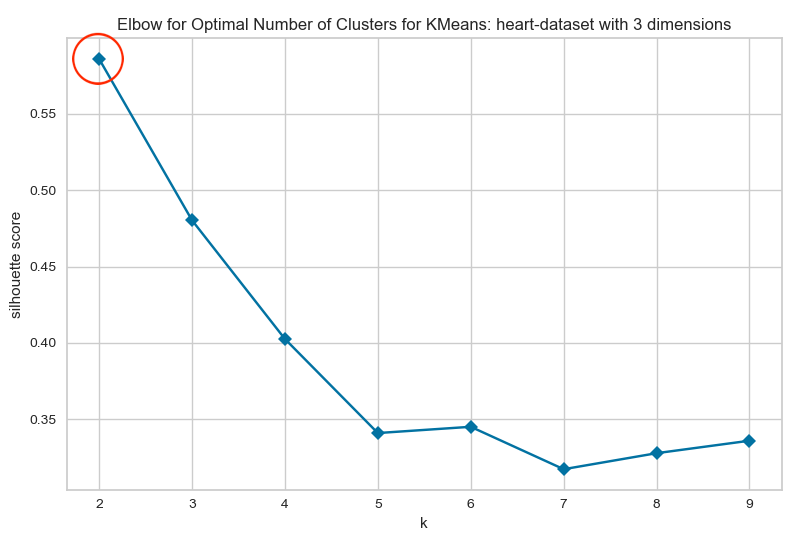
\includegraphics[width=0.75\textwidth]{Method/images/k-values/heart-dataset-3-kmeans.png}
  \caption{Selecting the $k$ for K-Means clustering for Heart dataset (3 dimensions) using the "silhouette method"}
  \label{hyperparameters:agglomerative-heart-dataset-3d}
\end{figure}
\begin{figure}[H]
  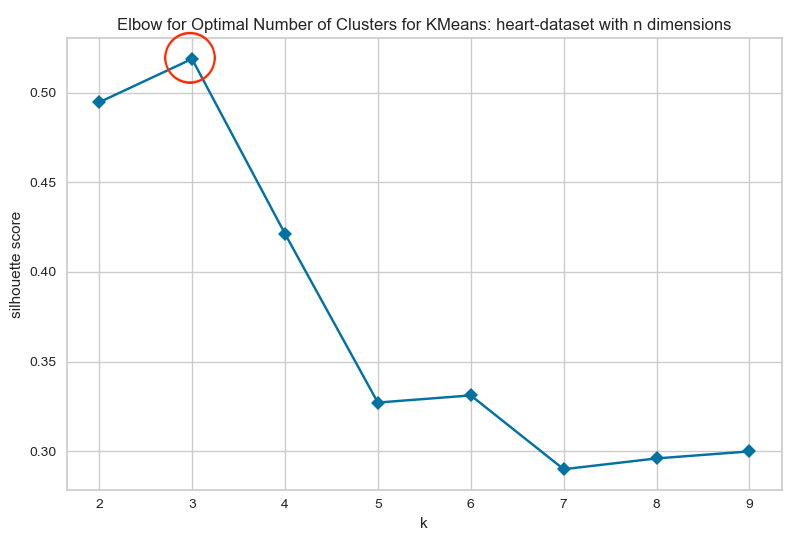
\includegraphics[width=0.75\textwidth]{Method/images/k-values/heart-dataset-n-kmeans.png}
  \caption{Selecting the $k$ for K-Means clustering for Heart dataset (9 dimensions) using the "silhouette method"}
  \label{hyperparameters:agglomerative-heart-dataset-9d}
\end{figure}
\newpage

\subsection{Circle dataset}

\begin{figure}[H]
  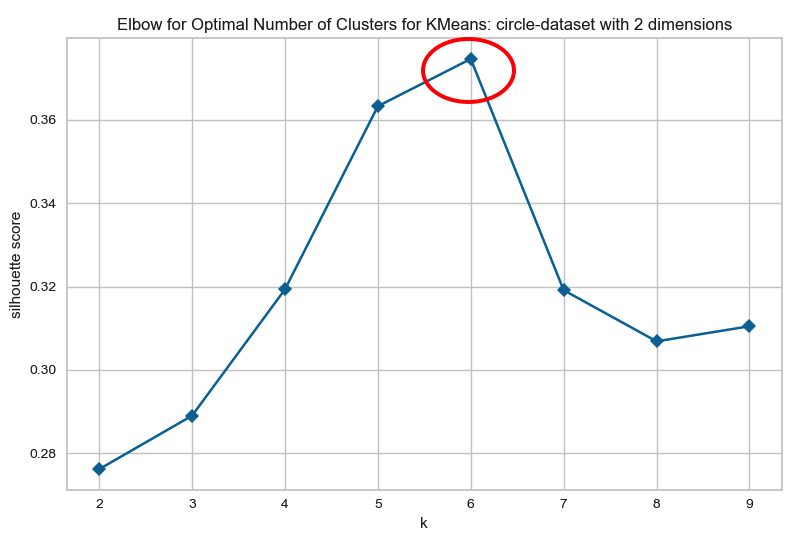
\includegraphics[width=0.75\textwidth]{Method/images/k-values/circle-dataset-2-kmeans.png}
  \caption{Selecting the $k$ for K-Means clustering for circle dataset (2-dimensions) using the "silhouette method"}
  \label{hyperparameters:agglomerative-circle-dataset-2d}
\end{figure}
\begin{figure}[H]
  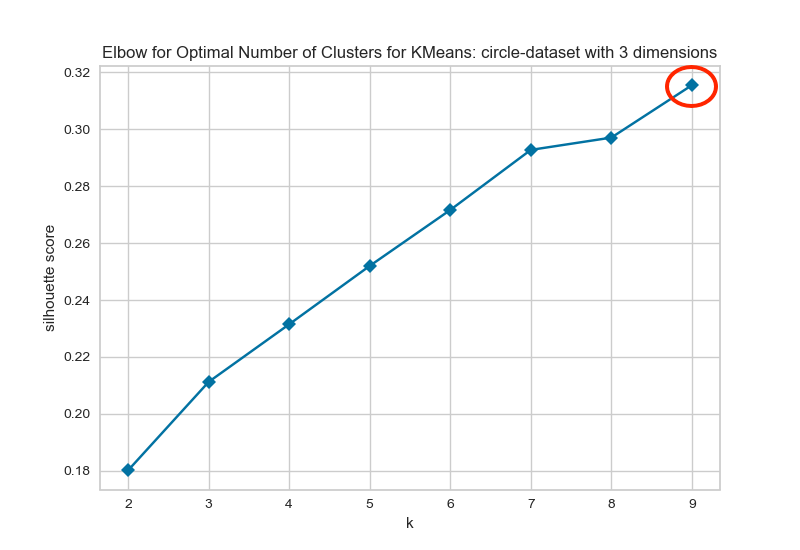
\includegraphics[width=0.75\textwidth]{Method/images/k-values/circle-dataset-3-kmeans.png}
  \caption{Selecting the $k$ for K-Means clustering for circle dataset (3-dimensions) using the "silhouette method"}
  \label{hyperparameters:agglomerative-circle-dataset-3d}
\end{figure}
\newpage

\subsection{Line dataset}
\begin{figure}[H]
  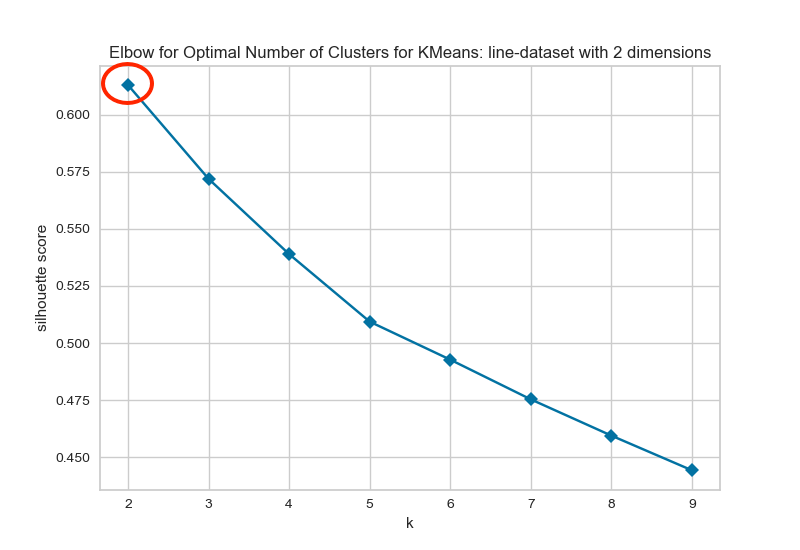
\includegraphics[width=0.75\textwidth]{Method/images/k-values/line-dataset-2-kmeans.png}
  \caption{Selecting the $k$ for K-Means clustering for line dataset (2-dimensions) using the "silhouette method"}
  \label{hyperparameters:agglomerative-line-dataset-2d}
\end{figure}
\begin{figure}[H]
  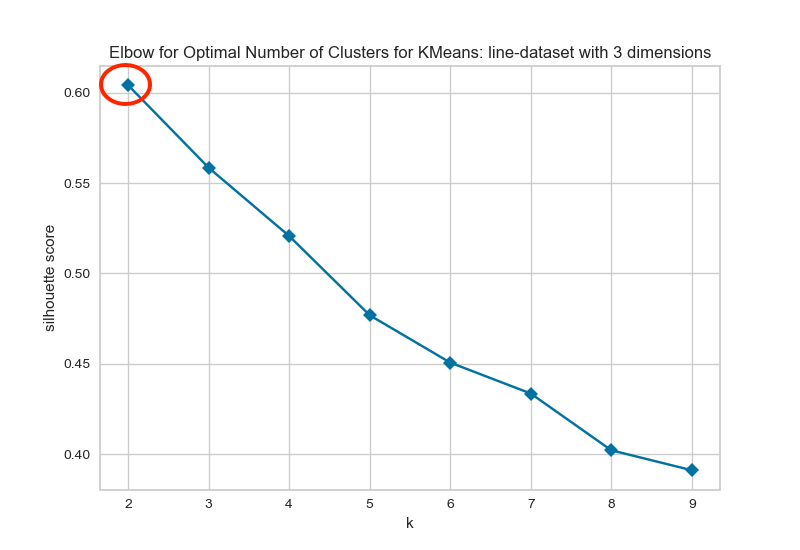
\includegraphics[width=0.75\textwidth]{Method/images/k-values/line-dataset-3-kmeans.png}
  \caption{Selecting the $k$ for K-Means clustering for line dataset (3-dimensions) using the "silhouette method"}
  \label{hyperparameters:agglomerative-line-dataset-3d}
\end{figure}
\newpage
\subsection{Skewed dataset}
\begin{figure}[H]
  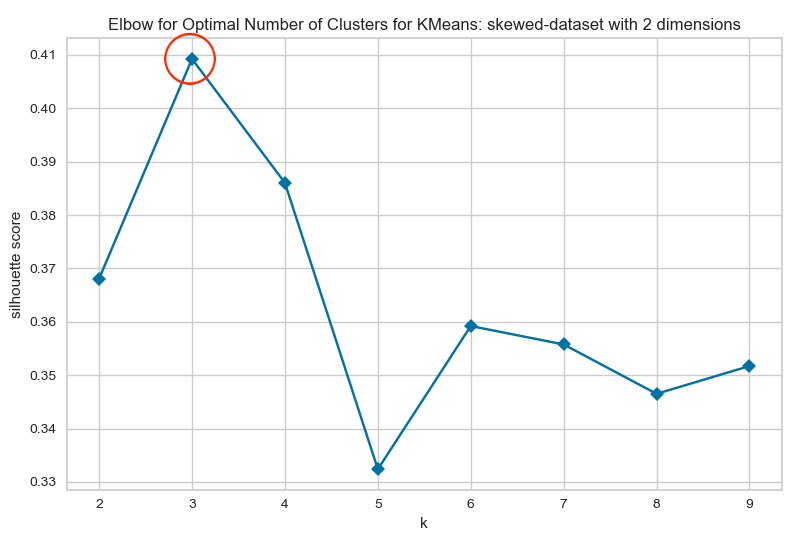
\includegraphics[width=0.75\textwidth]{Method/images/k-values/skewed-dataset-2-kmeans.png}
  \caption{Selecting the $k$ for K-Means clustering for skewed dataset (2-dimensions) using the "silhouette method"}
  \label{hyperparameters:agglomerative-skewed-dataset-2d}
\end{figure}
\begin{figure}[H]
  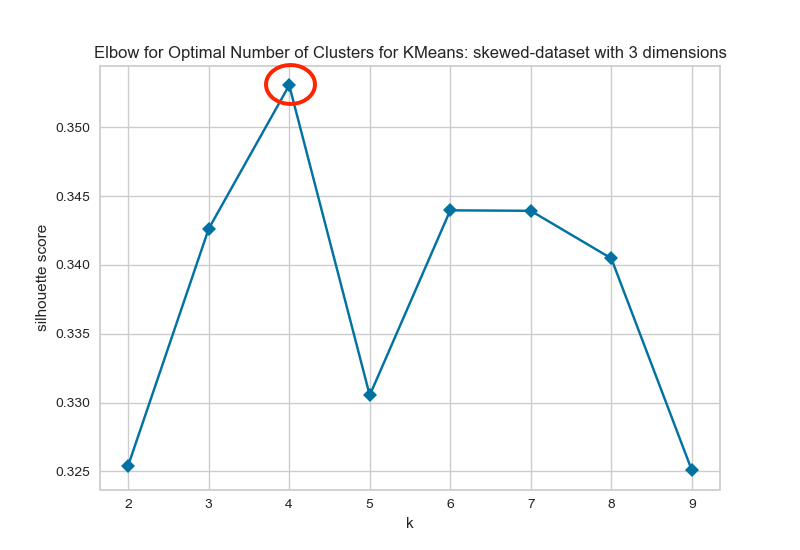
\includegraphics[width=0.75\textwidth]{Method/images/k-values/skewed-dataset-3-kmeans.png}
  \caption{Selecting the $k$ for K-Means clustering for skewed dataset (3-dimensions) using the "silhouette method"}
  \label{hyperparameters:agglomerative-skewed-dataset-3d}
\end{figure}
\newpage
\section{Agglomerative clustering} \label{appendix:agglomerative-hyperparameters}
The same as with K-Means applies to \gls{ag}.
\begin{enumerate}
    \item Seeds dataset:
    \begin{enumerate}
        \item 2-dimensions k-value: 2
        \item 3-dimensions k-value: 2
        \item 7-dimensions k-value 4
    \end{enumerate}
    \item     Heart dataset:
    \begin{enumerate}
        \item 2-dimensions k-value: 2
        \item 3-dimensions k-value: 4
        \item 9-dimensions k-value 3
    \end{enumerate}
    \item Circle dataset:
    \begin{enumerate}
        \item 2-dimensions k-value: 7
        \item 3-dimensions k-value: 9
    \end{enumerate}
    \item Line dataset (all dimensions) k-value: 
    \begin{enumerate}
        \item 2-dimensions k-value: 2
        \item 3-dimensions k-value: 3
    \end{enumerate}
    \item Skewed dataset:
    \begin{enumerate}
        \item 2-dimensions k-value: 6
        \item 3-dimensions k-value: 9
    \end{enumerate}
\end{enumerate}
\newpage
\subsection{Seeds dataset}
\begin{figure}[H]
  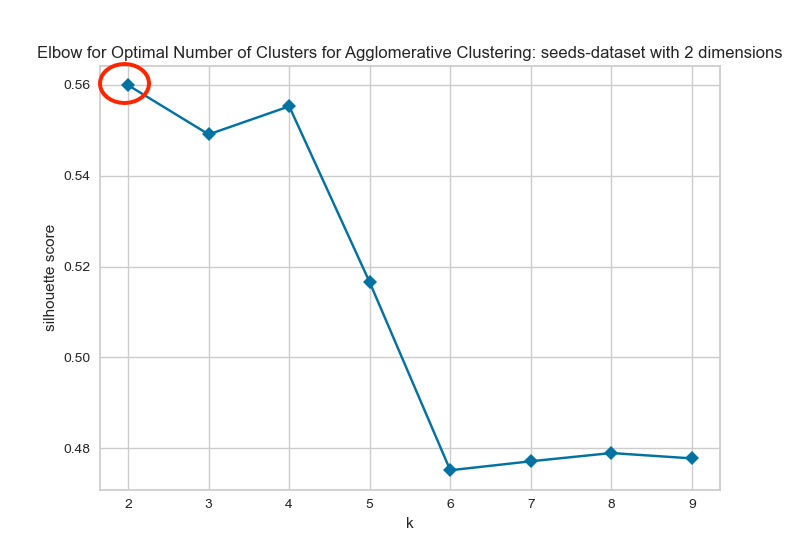
\includegraphics[width=0.75\textwidth]{Method/images/k-values/seeds-dataset-2-agglomerative.png}
  \caption{Selecting the $k$ for Agglomerative clustering for seeds dataset (2 dimensions) using the"silhouette method"}
  \label{hyperparameters:agglomerative-seeds-dataset-2d}
\end{figure}
\begin{figure}[H]
  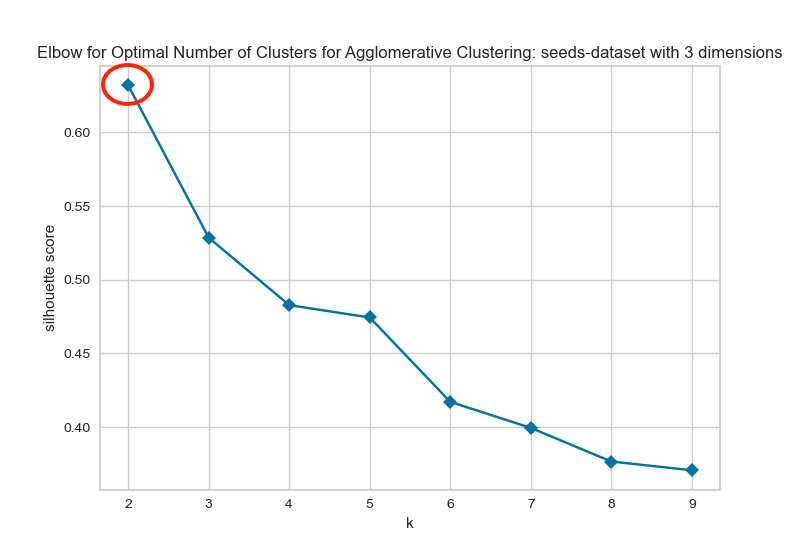
\includegraphics[width=0.75\textwidth]{Method/images/k-values/seeds-dataset-3-agglomerative.png}
  \caption{Selecting the $k$ for Agglomerative clustering for seeds dataset (3 dimensions) using the "silhouette method"}
  \label{hyperparameters:agglomerative-seeds-dataset-3d}
\end{figure}
\begin{figure}[H]
  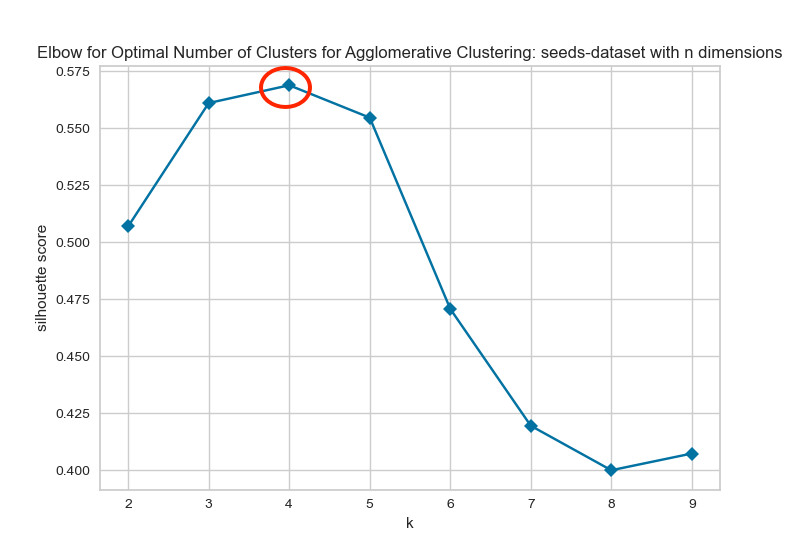
\includegraphics[width=0.75\textwidth]{Method/images/k-values/seeds-dataset-n-agglomerative.png}
  \caption{Selecting the $k$ for Agglomerative clustering for seeds dataset (7 dimensions) using the "silhouette method"}
  \label{hyperparameters:agglomerative-seeds-dataset-7d}
\end{figure}
\newpage

\subsection{Heart dataset}
\begin{figure}[H]
  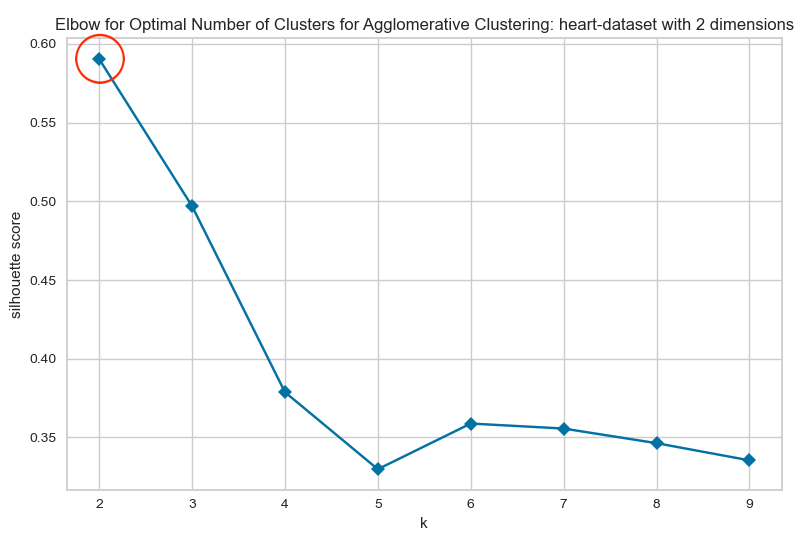
\includegraphics[width=0.75\textwidth]{Method/images/k-values/heart-dataset-2-agglomerative.png}
  \caption{Selecting the $k$ for Agglomerative clustering for Heart dataset (2 dimensions) using the "silhouette method"}
  \label{hyperparameters:agglomerative-heart-dataset-2d}
\end{figure}
\begin{figure}[H]
  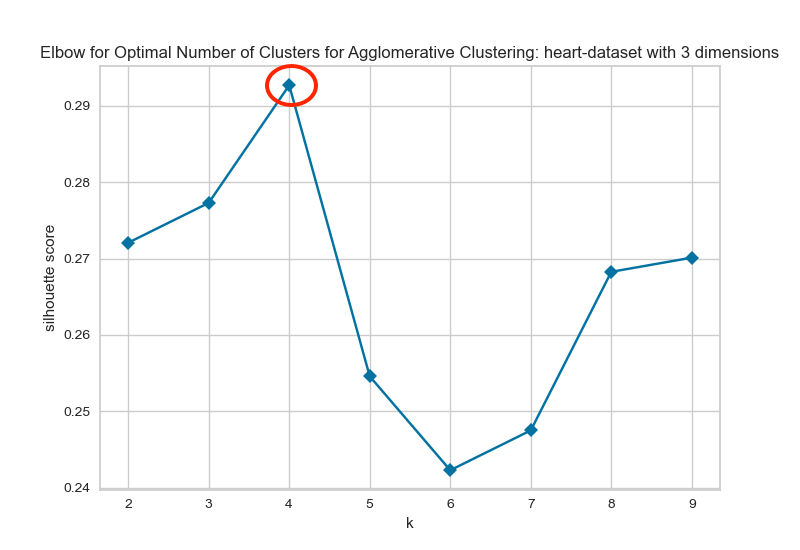
\includegraphics[width=0.75\textwidth]{Method/images/k-values/heart-dataset-3-agglomerative.png}
  \caption{Selecting the $k$ for Agglomerative clustering for Heart dataset (3 dimensions) using the "silhouette method"}
  \label{hyperparameters:agglomerative-heart-dataset-3d}
\end{figure}
\begin{figure}[H]
  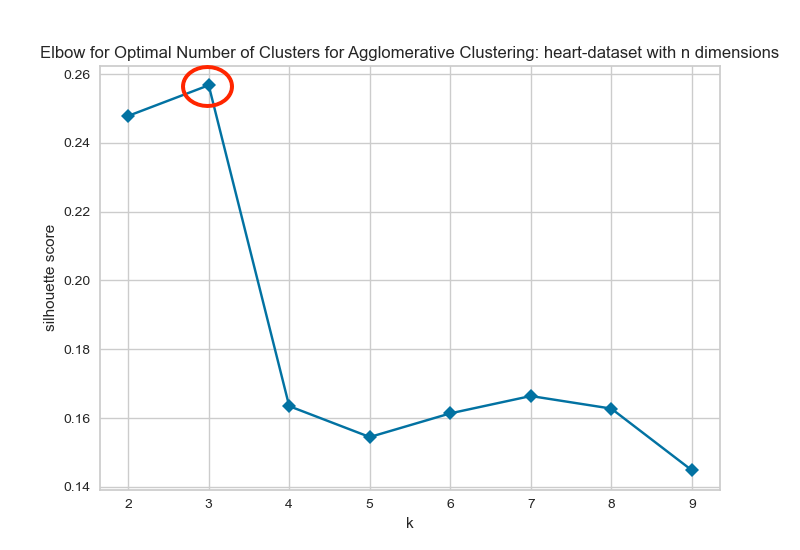
\includegraphics[width=0.75\textwidth]{Method/images/k-values/heart-dataset-n-agglomerative.png}
  \caption{Selecting the $k$ for Agglomerative clustering for Heart dataset (9 dimensions) using the "silhouette method"}
  \label{hyperparameters:agglomerative-heart-dataset-9d}
\end{figure}
\newpage

\subsection{Circle dataset}

\begin{figure}[H]
  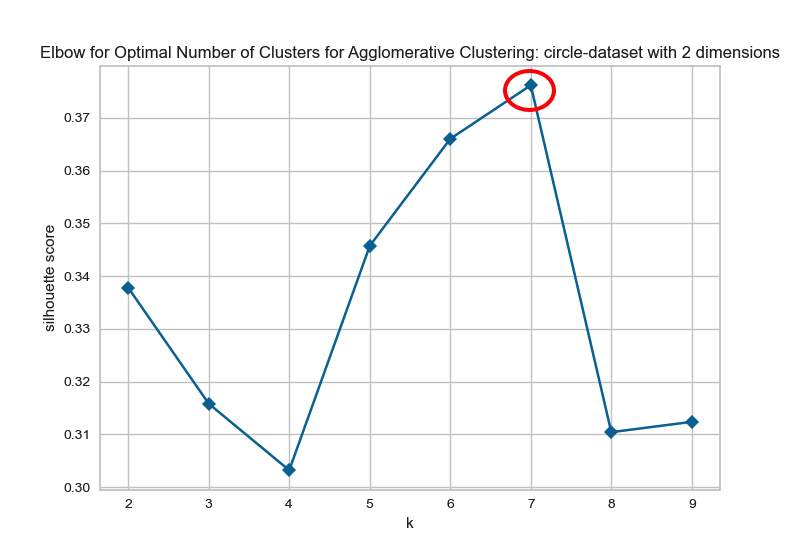
\includegraphics[width=0.75\textwidth]{Method/images/k-values/circle-dataset-2-agglomerative.png}
  \caption{Selecting the $k$ for Agglomerative clustering for circle dataset (2-dimensions) using the "silhouette method"}
  \label{hyperparameters:agglomerative-circle-dataset-2d}
\end{figure}
\begin{figure}[H]
  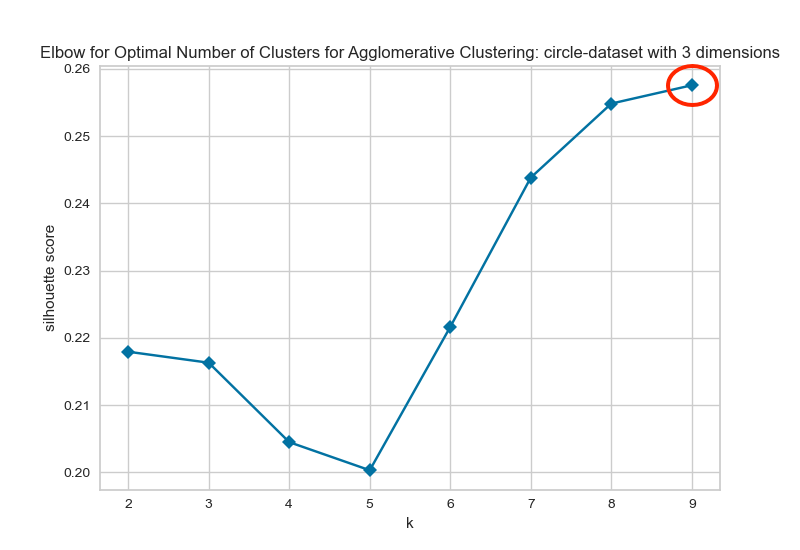
\includegraphics[width=0.75\textwidth]{Method/images/k-values/circle-dataset-3-agglomerative.png}
  \caption{Selecting the $k$ for Agglomerative clustering for circle dataset (3-dimensions) using the "silhouette method"}
  \label{hyperparameters:agglomerative-circle-dataset-3d}
\end{figure}
\newpage

\subsection{Line dataset}
\begin{figure}[H]
  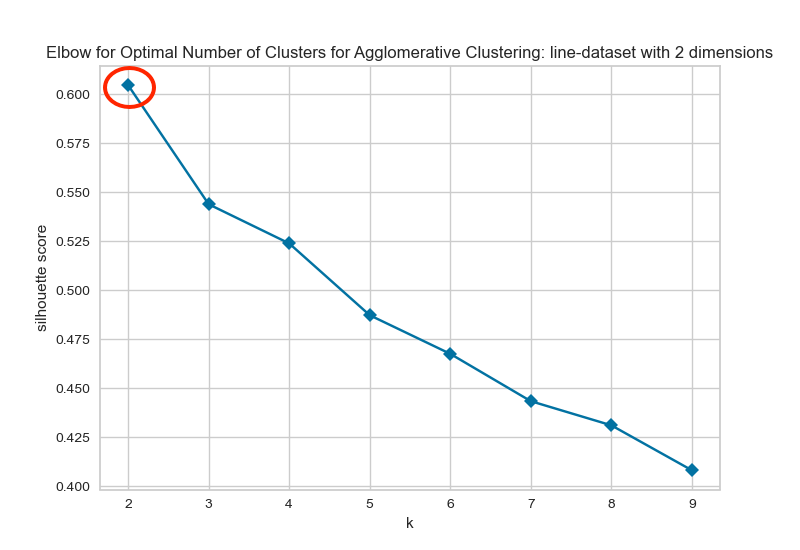
\includegraphics[width=0.8\textwidth]{Method/images/k-values/line-dataset-2-agglomerative.png}
  \caption{Selecting the $k$ for Agglomerative clustering for line dataset (2-dimensions) using the "silhouette method"}
  \label{hyperparameters:agglomerative-line-dataset-2d}
\end{figure}
\begin{figure}[H]
  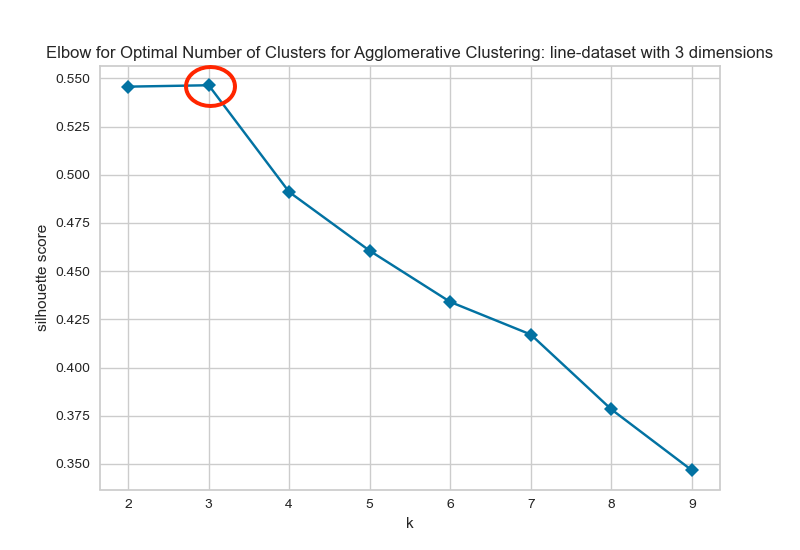
\includegraphics[width=0.75\textwidth]{Method/images/k-values/line-dataset-3-agglomerative.png}
  \caption{Selecting the $k$ for Agglomerative clustering for line dataset (3-dimensions) using the "silhouette method"}
  \label{hyperparameters:agglomerative-line-dataset-3d}
\end{figure}
\newpage
\subsection{Skewed dataset}
\begin{figure}[H]
  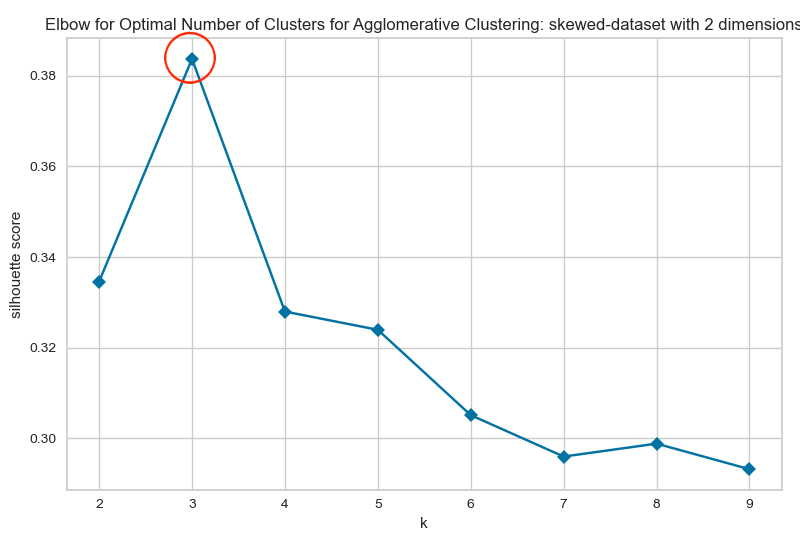
\includegraphics[width=0.75\textwidth]{Method/images/k-values/skewed-dataset-2-agglomerative.png}
  \caption{Selecting the $k$ for Agglomerative clustering for skewed dataset (2-dimensions) using the "silhouette method"}
  \label{hyperparameters:agglomerative-skewed-dataset-2d}
\end{figure}
\begin{figure}[H]
  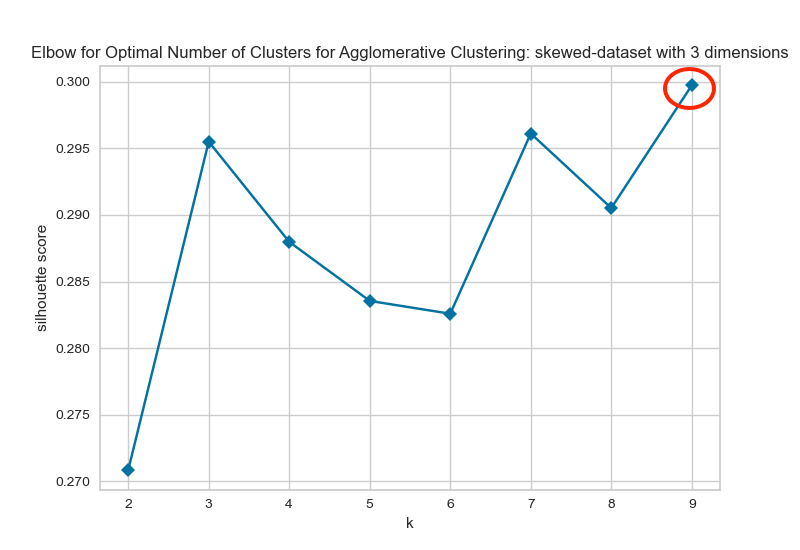
\includegraphics[width=0.75\textwidth]{Method/images/k-values/skewed-dataset-3-agglomerative.png}
  \caption{Selecting the $k$ for Agglomerative clustering for skewed dataset (3-dimensions) using the "silhouette method"}
  \label{hyperparameters:agglomerative-skewed-dataset-3d}
\end{figure}
%  \input{Appendices/appendix-b}
%  \input{Appendices/appendix-c}


\end{document}
